
% \addtocontents{toc}{\protect\newpage}
\section{Supervised Approaches}\label{sec:supervised-approaches}

The subsequent chapter frames trade classification as a supervised learning problem and has the primary focus on two learning methods: the tree-based ensemble gradient boosting and the deep learning-based FT-Transformer. We derive their suitability for trade classification through a concise discussion and explore both methods in detail.

\subsection{Framing as a Supervised Learning Problem}\label{sec:problem-framing}

All trade classification rules from \cref{sec:rule-based-approaches} perform discrete classification and assign a class to the trade. They are inherently unsupervised. Our focus is on supervised classification, where a classifier learns a function mapping between the input and the label, which represents the trade initiator.

More insightful, is to not just obtain the most probable class, but also the associated class probabilities for a trade to be a buy or sell. This gives insights into the quality of the prediction.
Thus, we frame trade signing as a supervised, probabilistic classification task. This is similar to \textcite[][272]{easleyDiscerningInformationTrade2016}, who alter the tick rule and \gls{BVC} algorithm to obtain the probability estimates of a buy from an individual or aggregated trades, but with a sole focus on trade signing on a trade-by-trade basis and supervised. For machine learning-based classifiers, a probabilistic view enables a richer evaluation but restricts the selection of classifiers. Trade classification rules, as presented in \cref{sec:rule-based-approaches}, do not profit from this alternative formulation as they yield hard probabilities only and so no insight into the confidence of the prediction is gained.

We introduce more notation, which is used throughout. Each data instance consists of a feature vector and the target. The former is given by $\mathbf{x} \in \mathbb{R}^{1 \times M}$ and described by a random variable $X$. Any of the $M$ features in $\mathbf{x}$ may be numerical, e.g., the trade price or categorical e.g., the security type. Like before, the target is given by $y \in \mathcal{Y}$ and described by a random variable $Y$. Each data instance is sampled from a joint probability distribution $\Pr(X, Y)$. The labelled data set with $N$ i.i.d. samples is denoted by $\mathcal{D} =\left\{\left(\mathbf{x}_i, y_i\right)\right\}_{i=1}^N$. For convienience, we define a feature matrix $\mathbf{X}=\left[\mathbf{x}_1,\ldots, \mathbf{x}_N\right]^{\top}$, that stores all instances and a corresponding vector of labels $\mathbf{y}=\left[y_1,\ldots, y_N \right]^{\top}$.

For our machine learning classifiers, we aim to model $\Pr_{\theta}(y \mid \mathbf{x})$ by fitting a classifier with the parameters $\theta$ on the training set. Given the estimated class probabilities, we retrieve the most probable class in $\mathcal{Y}$ as:
\begin{equation}
    \hat{y}=\arg\max_{y \in \mathcal{Y}} \operatorname{Pr}(y \mid \mathbf{x}).
    \label{eq:class-from-prob}
\end{equation}
\cref{eq:class-from-prob} allow alternating between a discrete and probabilistic formulation for trade classification. This enables a seamless comparison of classical rules and probabilistic classifiers in machine learning.
Next, we discuss state-of-the-art classifiers suitable for trade classification.

\subsection{Selection of Approaches}\label{sec:selection-of-approaches}

In this thesis, we perform a succinct literature discussion to select a set of supervised classifiers based on empirical evidence. In anticipation of the results, we ultimately select the FT-Transformer and Gradient Boosting for trade classification. To guide our discussion, we establish the following requirements a classifier must fullfil:
\begin{enumerate}[label=(\roman*),noitemsep]
\item \emph{performance:} The approach must deliver state-of-the-art performance in tabular classification tasks. Trades are typically provided as tabular datasets, consisting of rows representing instances and columns representing features. The classifier must be well-suited for probabilistic classification on tabular data.
\item \emph{scalability:}  The approach must scale to datasets with > 10~Mio. samples. Due to the high trading activity and long data history, datasets may comprise millions of samples, so classifiers must cope with large quantities of trades.
\item \emph{extensibility:} The approach must be extendable to train on partially-labelled trades.
\end{enumerate}

Trade classification, as we framed it, fits into supervised learning on tabular data, which is comprehensively covered by the research community with several studies reviewing and benchmarking newly proposed approaches against established machine learning methods.

\textbf{Wide Tree-Based Ensembles}

Traditionally, tree-based ensembles, in particular, \gls{GBRT} have dominated modelling on tabular data concerning predictive performance \autocites[][24--25]{grinsztajnWhyTreebasedModels2022}[][7]{kadraWelltunedSimpleNets2021}[][8]{gorishniyRevisitingDeepLearning2021}. At its core, tree-based ensembles combine the estimates of individual decision trees into an ensemble to obtain a more accurate prediction. For \gls{GBRT} \autocite[][9]{friedmanGreedyFunctionApproximation2001} the ensemble is constructed by sequentially adding small-sized trees into the ensemble that improve upon the error of the previous trees. Conceptually related to \glspl{GBRT} are random forests. Random forests \autocite[][6]{breimanRandomForests2001} fuse decision trees with the bagging principle \autocite[][123]{breimanBaggingPredictors1996} by growing multiple deep decision trees on random subsets of data and aggregating the individual estimates. 

\textcite[][7-9]{grinsztajnWhyTreebasedModels2022} trace back the strong performance of tree-based ensembles in tabular classification tasks to being a non-rotationally-invariant learner and tabular data being non-invariant to rotation. By intuition, rows and columns in a tabular dataset may be arranged in an arbitrary order, but each features carries a distinct meaning, which implies that feature values cannot be simply rotated without affecting the overall meaning. Thus, tabular data is non-invariant by rotation. So are tree-based ensembles, as they attend to each feature separately. This property also strengthens the model's ability to uninformative features \autocite[][8-9]{grinsztajnWhyTreebasedModels2022}.

\textcite[][13--14]{ronenMachineLearningTrade2022} have unparalleled success in classifying trades through random forests. Due to the framing as a probabilistic classification task, random forests are not optimal. This is because decision trees yield poorly calibrated probability estimates caused by limited samples in leaf nodes, which propagate to the ensemble \autocite[][356--360]{tanhaSemisupervisedSelftrainingDecision2017}. Gradient boosting is unaffected by this problem, and scales to large data sets due to the availability of highly optimised implementations that approximate the construction of ensemble members and can simultaneously learn from labelled and unlabelled instances. The state-of-the-art performance in tabular classification tasks, together with its ability to scale and extend, renders it suitable for trade classification.


\textbf{Deep Neural Networks}

Neural networks have emerged as powerful models for tabular data with several publications claiming to surpass \glspl{GBRT} in terms of performance. For brevity, we focus on two lines of research: regularised networks and attention-based networks, which have accumulated significant interest in the field. A recent overview of tabular deep learning can be found in \textcite[][1--22]{borisovDeepNeuralNetworks2022}.

\emph{Regularised Networks}

Among the simplest neural networks are \glspl{MLP}, which consists of multiple linear layers with non-linear activation functions in between. \textcite[][9--10]{kadraWelltunedSimpleNets2021} among others, advocate for the use of vanilla \gls{MLP} with an extensive mix of regularisation techniques, such as dropout \autocite{srivastavaDropoutSimpleWay} or residual connections \autocite{heDeepResidualLearning2015}, and report performance improvements over complex tabular-specific architectures or \glspl{GBRT}. Regularisation is expected to enhance generalisation performance, but the benefit is non-exclusive to \gls{MLP}. Conversely, when regularisation is equally applied to tabular-specific architectures, the effect reverses and multiple works including \textcites[][7]{gorishniyRevisitingDeepLearning2021}[][5]{grinsztajnWhyTreebasedModels2022} suggest that regularised \gls{MLP} actually trail the performance of specialised tabular-specific architectures. Also, \glspl{MLP} are rotatinally-invariant learners, as showed in \textcite[][5]{grinsztajnWhyTreebasedModels2022}, which contradicts our reasoning from above. To meet our performance criterion we instead focus on specialised architectures, particularly attention-based networks, while still emphasising the importance of a careful regularisation and optimisation.

\emph{Attention-based Networks}

Another emerging strand of research focuses on neural networks with an attention mechanism. Attention, intuitively, allows gathering information from the immediate context and learn relationships between features or between features and instances. It is incorporated in various architectures, including the tree-like TabNet \autocite[][3--5]{arikTabnetAttentiveInterpretable2020}, and several Transformer-based architectures including TabTransformer \autocite[][2--3]{huangTabTransformerTabularData2020}, Self-Attention and Intersample Attention Transformer \autocite[][4--5]{somepalliSaintImprovedNeural2021}, Non-Parametric Transformer \autocite[][3--4]{kossenSelfAttentionDatapointsGoing2021}, and FT-Transformer \autocite[][4--5]{gorishniyRevisitingDeepLearning2021}.

TabNet \autocite[][3--5]{arikTabnetAttentiveInterpretable2020}, fuses the concept of decision trees with attention. Similar to growing a decision tree, several sub-networks are used to process the input in a sequential, hierarchical fashion. Sequential attention, a variant of attention, is used to decide which features to select in each step. The output of TabNet is the aggregate of all sub-networks. Its poor performance in independent comparisons e.g., \textcites[][7]{kadraWelltunedSimpleNets2021}[][7]{gorishniyRevisitingDeepLearning2021}, raises doubts about its usefulness.

The Self-Attention and Intersample Attention Transformer uses a specialised attention mechanism, the intersample attention, to perform attention over both columns and rows \autocite[][4--5]{somepalliSaintImprovedNeural2021}. Applied to our setting, the model would contextualise information from the trade itself, but also from neighbouring trades, which is an unfair advantage over classical trade classification rules. Similarly, the Non-Parametric Transformer of \textcite[][3--4]{kossenSelfAttentionDatapointsGoing2021} uses the entire data set as a context, which rules out the application in our work.

Differently, TabTransformer \autocite[][2--3]{huangTabTransformerTabularData2020} performs attention per sample on categorical features-only. All numerical features are processed in a separate stream, a \gls{MLP}, which breaks correlations between categorical and numerical features \autocite[][2]{somepalliSaintImprovedNeural2021}. Most importantly though, most features in trade datasets are numerical. As such, trade classification would hardly profit from the Transformer architecture, causing the model to collapse to a vanilla \gls{MLP}. A more comprehensive approach is provided by \textcite[][4--5]{gorishniyRevisitingDeepLearning2021} in the form of FT-Transformer, that processes both numerical inputs and categorical input in Transformer blocks featuring an attention mechanism. Since it achieved state-of-the-art performance in independent empirical studies, like \textcite[][5]{grinsztajnWhyTreebasedModels2022}, and is non-rotationally invariant, we further consider FT-Transformer in our empirical study. Being based on the Transformer architecture, FT-Transformer naturally scales to large amounts of data and can utilise unlabelled data through self-training procedures.

The findings of \textcite[][50]{ronenMachineLearningTrade2022} do not support the use of neural networks in trade classification. But due to the lack of details regarding the model architecture, regularisation techniques, and training insights, it is necessary to reevaluate these findings in the context of option trades.

To summarise, our study considers gradient boosting and the FT-Transformer, each trained on labelled or partially-labelled trades. This comparison is particularly appealing, as it enables a multi-faceted comparison of wide tree-based ensembles versus deep neural networks, as well as supervised versus semi-supervised methods.

\subsection{Gradient Boosted Trees}\label{sec:gradient-boosted-trees}

This chapter first introduces decision trees and then combines individual trees in the gradient boosting procedure.

\subsubsection{Decision Tree}\label{sec:decision-tree}

Decision trees can be used in classification and regression. Despite solving a classification task, our focus is solely on regression trees, as it is the prevailing prediction model used in the gradient boosting algorithm \autocite[][9]{friedmanAdditiveLogisticRegression2000}. For this section, assume $y_i \in \mathbb{R}$.

A decision tree splits the feature space into several disjoint regions $R$ through a sequence of recursive splits. For a binary decision tree, a single split leads to two new sub-regions, whose shape is determined by the features considered for splitting and the preceding splits. Trees are grown in depth until a minimum threshold for the number of samples within a node or some other stopping criterion applies \autocite[][42]{breimanClassificationRegressionTrees2017}.
A region corresponds to a terminal node in the tree. For each terminal node of the tree or unsplit region, the predicted response value is constant for the entire region and shared by all its samples \autocite[][229]{breimanClassificationRegressionTrees2017}.

For a tree with $J$ regions $R_1, R_2,\ldots, R_J$, and some numerical input $\mathbf{x}$ the tree can be modelled as:
\begin{equation}
    h(\mathbf{x})=\sum_{j=1}^{J} \gamma_{j} \mathbb{I}\left(\mathbf{x} \in R_{j}\right),
    \label{eq:decision-tree}
\end{equation}
where $\mathbb{I}$ is the indicator function for region conformance and $\gamma_j$ the region's constant \autocite[][326]{hastietrevorElementsStatisticalLearning2009}. In the regression case, $\gamma_j$ is the mean of all target variables $y_i$ in the specific region. Since all samples of a region share a common response value, the tree estimates resemble a histogram that approximates the true regression surface, as visualised in \cref{fig:decision-boundary-dt}.

\begin{figure}[ht]
    \centering
    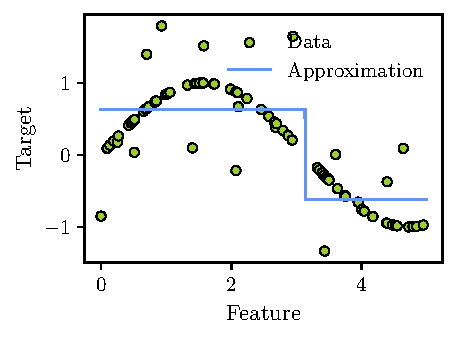
\includegraphics{decision-boundary-dt.pdf}
    \caption[Approximation of Decision Tree]{Approximation of a Decision Tree. A single split is performed at $\approx\num{3.1327505111694336}$ using the feature. All datapoints left respecitvely right of the split point share the region and are approximated by the region's response value.}
    \label{fig:decision-boundary-dt}
\end{figure}

So far, it remains open how the best split can be found. The best split is where the deviation between the prediction and the true response variable diminishes. For a single region, this error can be captured in the \gls{SSE} given by:
\begin{equation}
    \operatorname{L}_{\mathrm{SSE}} =\sum_{\mathbf{x}_{i} \in R_j}\left(y_{i}-\gamma_{j}\right)^{2},
\end{equation}
which is subsequently minimised \autocite[][231]{breimanClassificationRegressionTrees2017}. As documented in \textcite[][326]{hastietrevorElementsStatisticalLearning2009} we start with the entire dataset and scan through all combinations of features and possible split values. For a split by the feature $k$ at the value $s$, the child nodes are given by a pair of half-planes:
\begin{equation}
    R_1(k, s)=\left\{X \mid X_k \leq s\right\} \text { and } R_2(k, s)=\left\{X \mid X_k>s\right\}.
\end{equation}
Thereby, the feature $k$ and value $s$ are selected in a way, that the squared error in the child nodes is minimised:
\begin{equation}
    \min _{k, s}\left[\min _{\gamma_1} \sum_{\mathbf{x}_i \in R_1(k, s)}\left(y_i-\gamma_1\right)^2+\min _{\gamma_2} \sum_{\mathbf{x}_i \in R_2(k, s)}\left(y_i-\gamma_2\right)^2\right].
\end{equation}
Clearly, growing deeper trees leads to an improvement in the \gls{SSE}. Considering the extreme, where each sample has its region, the tree would achieve a perfect fit in-sample but perform poorly on out-of-sample data. To reduce the sensitivity of the tree to changes in the training data, hence \emph{variance}, size complexity pruning procedures are employed. Likewise, if the decision tree is too simplistic, a high bias contributes to the model's overall expected error. Both extremes are to be avoided.

Ensemble methods decrease the expected error of the decision tree by combining multiple trees in a single model through minimising the bias or variance term or both. Specifically, boosting addresses the bias and variance \autocites[][1672]{schapireBoostingMarginNew1998}[][29]{breimanRandomForests2001}. Next, we focus on \gls{GBRT}, a variant of boosting.

\subsubsection{Gradient Boosting
    Procedure}\label{sec:gradient-boosting-procedure}

Gradient boosting iteratively combines oversimplified models, the weak learners, into an additive model to obtain an improved ensemble estimate. This chapter draws on \textcite[][9]{friedmanGreedyFunctionApproximation2001} to derive gradient boosting for binary classification.

% classifier with outputs in [-1, 1]
By \cref{sec:problem-framing} we perform binary probabilistic classification and by \cref{sec:trade-initiator} we defined the labels to be $y \in \{-1,1\}$. For gradient boosting, instead of modelling the class-conditional probabilities directly, we model the conditional log odds instead, which can be interpreted as the probability of observing class $1$ or a buyer-initiated trade, and covert to class-conditional probabilities as needed.


\todo{better write logloss? Make connection clearer?}
Following \textcite[][9]{friedmanStochasticGradientBoosting2002} we set the loss function to be the cross-entropy loss, given by:
\begin{equation}
    L_{\mathrm{BCE}} \colon \mathbb{R}^2 \to \mathbb{R} \quad L_{\mathrm{BCE}}(y, F) = \log(1+\exp(-2yF))
    \label{eq:cross-entropy-loss}
\end{equation}
where:
\begin{equation}
    F(\mathbf{x}) = \frac{1}{2} \log \left[\frac{\Pr(y=1\mid \mathbf{x})}{\Pr(y=-1\mid \mathbf{x})}\right]
    \label{eq:logits-gbm}
\end{equation}
$F(\mathbf{x})$ is the model's prediction in terms of conditional log odds. The cross-entropy loss, is a reasonable choice, as it is suitable for binary classification, convex, and twice differentiable; properties we exploit later.

We first intialise the model with a naïve prediction, based on the average class $\bar{y}$ from all training samples:

\begin{equation}
    F_0(\mathbf{x})= \frac{1}{2} \log \left[\frac{1+\bar{y}}{1-\bar{y}}\right].
\end{equation}
Expectedly, $F_0(\mathbf{x})$ is a poor estimate, capturing hardly any regularities of the data. Gradient boosting solves this issue by adding weak learners to the ensemble. New trees are added greedily, one per iteration $m$ with $m=1,2,\cdots M$. The weak learner in the $m$-th iteration is chosen to approximate the pseudo residual $r_i$, which is the negative gradient of the observed value of the $i$-th sample and the current estimate:
\begin{equation}
    r_i=-\left[\frac{\partial L_{\mathrm{BCE}}\left(y_i, F\left(\mathbf{x}_i\right)\right)}{\partial F\left(\mathbf{x}_i\right)}\right]_{F(\mathbf{x})=F_{m-1}(\mathbf{x})}=2 y_i /\left(1+\exp \left(2 y_i F_{m-1}\left(\mathbf{x}_i\right)\right)\right).
\end{equation}
\todo{yields the maximum decrease are similar to the components of the negative gradient descent. However, the  major drawback is tha tthe gradient is only defined for data points xi seen during training, contradicting the creation of a generalising model.}
Typically, regression trees (cp. \cref{sec:decision-tree}) are chosen as weak learners since they are computationally cheap and can produce continuous estimates for the residual. The $m$-th regression tree contains $J$ terminal regions, denoted by $R_{j m}, j=1,2, \ldots, J_{m}$. We search for an estimate $\gamma_{j,m}$ for the terminal node $R_{jm}$ that minimises the cross-entropy over all samples within the node:
\begin{equation}
    \gamma_{j m}=\arg \min _\gamma \sum_{\mathbf{x}_i \in R_{j m}} \log \left(1+\exp \left(-2 y_i\left(F_{m-1}\left(\mathbf{x}_i\right)+\gamma\right)\right)\right)
    \label{eq:region-estimate-gbm}
\end{equation}

\cref{eq:region-estimate-gbm} cannot be solved in closed form and is typically approached by the Newton-Raphson method with a second-order approximation of the loss~\footnote{Compare the second-order Taylor polynomial given by \todo{complete?}.}:
\begin{equation}
    \gamma_{j m}=\sum_{\mathbf{x}_i \in R_{j m}} r_i / \sum_{\mathbf{x}_i \in R_{j m}}\left|r_i\right|\left(2-\left|r_i\right|\right)
\end{equation}
with $r_i$ given by \cref{eq:logits-gbm}.

An improved estimate for $\mathbf{x}$ is calculated from the previous estimate by adding the new regression tree to the ensemble. The latter moves the prediction towards the greatest descent and thus improves the overall prediction. The updated model is given by:
\begin{equation}
    F_{m}(\mathbf{x})=F_{m-1}(\mathbf{x})+\eta \sum_{j=1}^{J_{m}} \gamma_{j m} \mathbb{I}\left(\mathbf{x} \in R_{j m}\right).
\end{equation}
After $M$ iterations we obtain the final estimate calculated as $F_{M}\left(\mathbf{x}\right)$. To avoid \gls{overfitting} the residuals, only proportional steps towards the negative gradient are taken, which is controlled by the learning rate \eta~\autocite[][13]{friedmanGreedyFunctionApproximation2001}. The learning rate \eta~and the size of the ensemble $M$ are deeply intertwined and best tuned together \autocite[][13]{friedmanGreedyFunctionApproximation2001}.

Gradient boosting is still prone to \gls{overfitting} due to fitting trees to point-wise gradients. One solution is to employ early stopping, whereby the ensemble is only grown in size, as long as adding more weak learners leads to a decrease in loss on the validation set \autocite[][384]{hastietrevorElementsStatisticalLearning2009}. Another approach is to limit the amount of data seen during training by fitting trees on random subset of samples, as proposed in \textcite[][3]{friedmanStochasticGradientBoosting2002}, or on a subset of features, as popularised by \textcite[][3]{chenXGBoostScalableTree2016}. \textcite[][6]{prokhorenkovaCatBoostUnbiasedBoosting2018} grow oblivious trees, which use the same splitting criterion for all nodes of one level in a tree. The rationale is, that these arguably simplistic trees, and achieve an imperfect fit, which regularises the model. Finally, the loss function can be extended for a $\ell_2$ regularisation term to penalise the model for complexity \autocite[][2]{chenXGBoostScalableTree2016}.

In recent years, several variants of gradient boosting have been proposed and studied in the literature, including CatBoost \autocite[][1--23]{prokhorenkovaCatBoostUnbiasedBoosting2018}, XGBoost \autocite[][1--13]{chenXGBoostScalableTree2016}, and LightGBM \autocite[][3]{keLightGBMHighlyEfficient2017}, which differ by the policy how trees are grown and how \gls{overfitting} is addressed. Performance-wise, differences between the implementations are negligible, as empirical studies suggest \autocites[][8]{grinsztajnWhyTreebasedModels2022}[][19--20]{gorishniyRevisitingDeepLearning2021}[][7]{somepalliSaintImprovedNeural2021}[][14]{borisovDeepNeuralNetworks2022}.

As we noted at the beginning, $F_M(\mathbf{x})$ models the log odds. We can recover the class-conditional probabilities $\widehat{\operatorname{Pr}}(y \mid \mathbf{x})$ by taking the inverse:
\begin{equation}
    \widehat{\operatorname{Pr}}(y \mid \mathbf{x}) = 1 /\left(1+\exp(-2yF_M(\mathbf{x}))\right).
\end{equation}
and get the most probable class by \cref{eq:class-from-prob}.

\subsection{Transformer Networks}\label{sec:transformer-networks}

The subsequent chapters provide an introduction to classifiers based on the Transformer architecture.

\subsubsection{Architectural Overview}\label{sec:architectural-overview}

The Transformer is a neural network architecture by \textcite[][2--6]{vaswaniAttentionAllYou2017} proposed for sequence-to-sequence modelling. Its original application is in machine translation, whereby sentences in the source language are translated into sentences in the target language. More precisely, the sentence is first decomposed into individual \glspl{token} and mapped into a sequence of \glspl{embedding}, which are rich vector representations of the raw input. The Transformer then processes the \glspl{embedding} to generate the output sequence.

As the network operates on \glspl{embedding}, rather than strings, the architecture is not constrained to process textual data. It has been adapted to other modalities including image data \autocites[][2--5]{parmarImageTransformer2018}[][3]{dosovitskiyImageWorth16x162021} and tabular data \autocite[cp.][4]{gorishniyRevisitingDeepLearning2021}. The latter is important for our work, as derived in \cref{sec:selection-of-approaches}.

Following the architecture for machine translation of \textcite[][3]{sutskeverSequenceSequenceLearning2014}, the network features two main components: the encoder and the decoder. A sequence of \glspl{token} is first mapped to a sequence of \glspl{embedding} and augmented with positional information. The encoder receives these \glspl{embedding} and creates an enriched representation from it by encoding the context in which the input appears i.e., the surrounding words. The output of the encoder is then fed to the decoder. The decoder takes the embedded target sequence along with parts of the encoded representation of the input, to autoregressively generate the output sequence, i.e., the translation in the target language \gls{token} by \gls{token} \autocite[][3]{vaswaniAttentionAllYou2017}. \cref{fig:transformer-architecture-overview} depicts the complete architecture and serves as a guide through the subsequent sub-chapters.

The encoder consists of $\gls{L}=6$ stacked Transformer blocks \autocite[][6]{vaswaniAttentionAllYou2017}. Each block itself is composed of two sub-layers: a multi-head self-attention layer, followed by a position-wise, \gls{feed-forward-network}. Both components serve a distinct purpose in the Transformer. The self-attention mechanism encodes the context in which the input appears onto the \glspl{embedding}, whereas the \gls{feed-forward-network} serves as a long-term memory persisting information outside the immediate context. In the multi-head self-attention mechanism of the encoder, inputs can learn from any \gls{token} of the input sequence, even if a \gls{token} appears causally before the other input. Each of the sub-layers is surrounded by skip connections \autocite[][2]{heDeepResidualLearning2015} and followed by layer normalisation \autocite[][4]{baLayerNormalization2016} to facilitate and stabilise training. Stacking multiple Transformer blocks enables the model to learn hierarchical features from the inputs and targets. Applied to language processing, the first layers in the stack extract coarse-grained syntactic features, and subsequent layers learn fine-grained semantic features \autocites[][3651]{jawaharWhatDoesBERT2019}[][4596]{tenneyBERTRediscoversClassical2019}. For tabular data, this translates to frequent feature combinations or infrequent feature interactions.

Aside from the feed-forward sub-layer, the decoder contains a sub-layer for multi-head self-attention on the output of the encoder, known as cross-attention, and a masked variant of the multi-head self-attention for use on the output sequence. Here, causal masking enforces the autoregressive properties of the decoder.

The output of the decoder is finally passed through a linear layer with a softmax activation function to unembed the output and retrieve the probabilities of the next \gls{token} \autocite[][5]{vaswaniAttentionAllYou2017}. Since the output sequence is generated autoregressively, the most probable \gls{token} is fed back as input to the decoder to provide context for the following \glspl{token} until the remaining sequence is generated.

For its original application, machine translation, both the encoder and decoder are used. Yet, the modular design allows adapting Transformers to a wider range of use cases, some of which only require the encoder or decoder. \textcite[][16--17]{raffelExploringLimitsTransfer2020} differentiate these modes: encoder-only architecture, which encodes the input to obtain an enriched representation, decoder-only architectures to generate new \glspl{token} and encoder-decoder models for sequence-to-sequence modelling autoregressively. As our focus is on the probabilistic classification of tabular data, the goal is to learn an enriched representation of the input for classifying the label, here $\gls{y}$, rather than generating new samples. As such, encoder-only Transformers suffice. This insight also guides the structure in the next chapters, which focus on \glspl{embedding} and the inner workings of the encoder.

\begin{landscape}
    \begin{figure}[ht]
        \centering
        {\renewcommand\normalsize{\scriptsize}%
            \normalsize
            \input{./Graphs/transformer-architecture.pdf_tex}}
        \caption[Overview Over the Transformer Architecture]{Overview over the Transformer Architecture. The left part shows the self-attention mechanism discussed in \cref{sec:attention}. The central part depicts the multi-head self-attention mechanism, as covered in \cref{sec:attention}. The right part shows the encoder and decoder stack, as well as the \gls{embedding} mechanism as covered in \cref{sec:token-embeddings} onwards. Own work inspired by \textcite[][3]{tayEfficientTransformersSurvey2022}.}
        \label{fig:transformer-architecture-overview}
    \end{figure}
\end{landscape}

\subsubsection{Token Embedding}\label{sec:token-embeddings}

As explained previously, Transformers operate on sequences of numeric vector representations, the \emph{token embeddings}. The classical Transformer was trained on \emph{word embeddings}. Nevertheless, \gls{token} embeddings are generic and arbitrary inputs that can be embedded and then processed by the Transformer. In the spirit of \textcite[][5]{vaswaniAttentionAllYou2017}, we first explore word embeddings for textual data, before adapting embeddings to the tabular domain.

\todo{write down, how sequence of token ids is constructed.}

\textbf{Embeddings For Textual Data}

To obtain \gls{token} embeddings from the raw input sequences i.e., a sentence, the sequence is first split into constituent vocabulary elements, the \emph{tokens}. All known \glspl{token} are stored in a vocabulary. The vocabulary $V$ consists of $N_{V}=|V|$ elements and maps \glspl{token} onto their unique integer keys, referred to as \emph{token-ids} \autocite[][3]{phuongFormalAlgorithmsTransformers2022}. Apart from \glspl{token} in the training corpus, the vocabulary may include special \glspl{token}, like the $\mathtt{[UNK]}$ \gls{token} to handle out-of-vocabulary items or $\mathtt{[CLS]}$ \gls{token} for storing an aggregate representation of the sequence for classification \autocite[cp.][4]{devlinBERTPretrainingDeep2019}.

For ease of explanation, we equate \glspl{token} with words.\footnote{There is a subtle difference between \glspl{token} and words. A \gls{token} can be words including punctuation marks. But words can also be split into multiple \glspl{token}, such as sub-words \autocite[][3]{bojanowskiEnrichingWordVectors2017} or characters. To decrease the size of the vocabulary, words may be reduced to their stems, lower-cased, and stop words be removed.} Consider the following example with a small vocabulary of $V=\left\{1, N_v\right\}$ and a mapping between the \gls{token} and token-id of $\mathrm{'queen'}\mapsto 1$; $\mathrm{'king'}\mapsto 2$. For the sample sequence »Kings and Queens«, the sequence of token-ids is $\mathbf{s}=[2, 1]$, after applying tokenizing by words and common pre-processing like lower-casing, and the removal of the stop word »and«. Arbitrary sequences are given by $\mathbf{s} \equiv s[1: \ell] \equiv$ $s[1] s[2] \ldots s[\ell] \in V^*$.

The conversion to token-ids, however, loses the semantics, as token-ids may be assigned arbitrarily or ordering by semantics may not be feasible. This limitation can be overcome by embeddings, as pioneered by \textcite[][1139]{bengioNeuralProbabilisticLanguage}, which map each token-id into a high-dimensional space. By representing words as a vector, semantic and syntactic relationships between tokens can be encoded. As such, related words share a similar embedding vector \autocite[][1139]{bengioNeuralProbabilisticLanguage}. Moreover, word embeddings are semantically meaningful and can capture linguistic regularities, like gender through offsets between vectors \autocite[][748--749]{mikolovLinguisticRegularitiesContinuous2013}.

The embedding layer from \cref{fig:transformer-architecture-overview} is ultimately a lookup table to retrieve the embedding vector $\gls{e} \in \mathbb{R}^{d_{e}}$ from a learnt embedding matrix $\gls{W-e} \in \mathbb{R}^{d_{e} \times N_{V}}$ with the token-id $v \in V \cong\left[N_{V}\right]$ as shown:\footnote{Throughout our discussion on Transformers we adopt a notation proposed in \textcite[][1--16]{phuongFormalAlgorithmsTransformers2022}.}
\begin{equation}
    \gls{e}=\gls{W-e}\left[:, v\right].
    \label{eq:word-embeddings}
\end{equation}
The weights of $\gls{W-e}$ are initialised randomly and updated using gradient descent to obtain the learnt embeddings. The dimension of the embedding $d_e$ affects the expressiveness of the network and is thus an important tuneable hyperparameter of the model. All embeddings of the input sequence are finally gathered in a matrix $\mathbf{S} \in \mathbb{R}^{d_e \times \ell_s}$.

Concluding the example from above with artificial embeddings of $d_e=3$:
\begin{equation}
    \begin{aligned}
        \gls{e}_{\mathrm{king}}  & =\gls{W-e}\left[:,2\right] = [0.01, 0.20, 0.13]^{\top} \\
        \gls{e}_{\mathrm{queen}} & =\gls{W-e}\left[:,1\right] = [0.07, 0.16, 0.14]^{\top} \\
    \end{aligned}
\end{equation}
are likely to be close in embedding space with cosine-similarity of $\approx 1$ due to their high semantic similarity.

As this work is concerned with the classification of tabular data, the aforementioned concepts must be evolved. Differently from textual data, where all tokens come from the same vocabulary and a homogeneous embedding procedure suffices, tabular data is flexible regarding the columns, their data type, and their semantics. Only a shared meaning across rows can be assumed. For instance, every sample in a trade dataset may contain the previous trade price, yet the meaning of the trade price is different from other columns, urging the need for heterogeneous embeddings. Additionally, columns may be categorical or numerical.

\textbf{Embeddings For Numerical Data}

Transformer networks can handle numerical features, such as the trade price, by mapping the scalar value to a high-dimensional embedding vector and process sequences thereof \autocite[][3]{gorishniyEmbeddingsNumericalFeatures2022}. In the simplest case, a learnt linear projection is utilised to obtain the embedding. Linear embeddings of numerical features were previously explored in \textcites[][3]{kossenSelfAttentionDatapointsGoing2021}[][4]{somepalliSaintImprovedNeural2021}[][4]{gorishniyRevisitingDeepLearning2021}.

In analogon to the word case, if the $m$-th feature, $\mathbf{x}[m]$, is numerical, it is projected to its embedding $\gls{e} \in \mathbb{R}^{d_e}$ by element-wise multiplication with a learnt vector $\mathbf{W}_m \in \mathbb{R}^{d_{e}}$. Moreover, a feature-dependent bias term $\mathbf{b}_m \in \mathbb{R}^{d_{e}}$ is added, as noted in \cref{eq:numerical-embeddings}.
\begin{equation}
    \gls{e}= \mathbf{W}_m \mathbf{x}[m] +\mathbf{b}_m
    \label{eq:numerical-embeddings}
\end{equation}
More sophisticated approaches rely on parametric embeddings, like the \emph{piece-wise linear encoding} or the \emph{periodic encoding} of \textcite[][10]{gorishniyEmbeddingsNumericalFeatures2022}. Both enforce non-linearity. The authors show that these can alleviate the model's performance but at a non-neglectable computational cost. For this reason, our focus is on the computational more tractable linear embedding.

More generally, the works of \textcites[][1]{gorishniyEmbeddingsNumericalFeatures2022}[][1]{somepalliSaintImprovedNeural2021} suggest, that numerical embedding can significantly improve robustness to missing values or noise. Their work miss a theoretical explanation. \textcite[][8--9]{grinsztajnWhyTreebasedModels2022} fill this void and attribute the increased robustness to the broken rotational invariance.

\textbf{Embeddings For Categorical Data}

Datasets often comprise categorical features like the underlying. In the context of tabular Transformers, learnt categorical embeddings are widely used, which are similar to the word embedding
\autocites[][4]{gorishniyRevisitingDeepLearning2021}[][2]{huangTabTransformerTabularData2020}[][4]{somepalliSaintImprovedNeural2021}. Analogous, each category is mapped to an embedding vector using a learnt embedding matrix. Due to the heterogeneous nature of tabular data, embeddings may not be shared between features.

For categorical inputs, the embedding is implemented as a lookup table, analogous to \cref{eq:word-embeddings}. However, each feature has
its vocabulary $C_t$ with $N_{C_m}$ categories. Assume, the $m$-th feature is categorical. The specific embeddings $\gls{e}$ are queried with a unique integer key $c_{m} \in C_m \cong\left[N_{C_t}\right]$ from the learnt embedding matrix $\mathbf{W}_m \in \mathbb{R}^{d_e \times N_{C_m}}$. Finally, a feature-specific bias term $\mathbf{b}_m \in \mathbb{R}^{d_{e}}$ is added as shown in \cref{eq:categorical-embeddings}. Like for the word case, all embeddings of an instance are gathered in $\mathbf{S}$.
\begin{equation}
    \gls{e}=\mathbf{W}_m[:,c_{m}] +\mathbf{b}_m
    \label{eq:categorical-embeddings}
\end{equation}
These categorical embeddings can potentially capture the intrinsic properties of categorical variables by arranging similar categories closer in the embedding space. For instance, consider the underlyings $\mathtt{GOOGL}$ (Alphabet Inc.), $\mathtt{MSFT}$ (Microsoft Inc.), and $\mathtt{K}$ (Kellogg Company). Due to the overlapping field of operations, one would anticipate greater similarity between Alphabet and Microsoft.

Despite these advantages, high-cardinal features present a challenge for embeddings since they are typically learnt from a few samples, which promotes \gls{overfitting}. Handling high-dimensional categorical data remains an open research problem, as noted by \textcite[][2]{borisovDeepNeuralNetworks2022}.

\textbf{Link To Positional Encoding and Attention}

\todo{verify invariant property. Not sure if I got it right.}
Embeddings can only encode the semantic relationship of tokens, but they do not provide a clue to the model about the relative and absolute ordering of tokens in which they appear in the sequence, since all stages of the encoder and decoder are invariant to the token's position. Positional information must be induced into the model to preserve the ordering (cp. \cref{sec:positional-encoding}). Another limitation of embeddings is, that identical tokens share the embedding, even if they are ambiguous and their meaning is different from the context in which they appear. To resolve this issue, embeddings get contextualised in the self-attention mechanism (cp. \cref{sec:attention}).

\subsubsection{Positional Encoding}\label{sec:positional-encoding}

In practice, the order of words is important for the overall meaning of a sentence. As such, \textcite[][6]{vaswaniAttentionAllYou2017} propose to inject information on the \gls{token}'s position within the sequence through a \emph{positional encoding}, that is added onto the \gls{token} embedding.

Contrary to sentences, columns in tabular datasets are arranged in an arbitrary order, which weakens the need for positional information. However, unless the embeddings per feature are unique, a positional embedding is also required so that the model can relate the otherwise identical embeddings to specific features and distinguish them \autocites[][3]{huangTabTransformerTabularData2020}[][15]{somepalliSaintImprovedNeural2021}.

Like \gls{token} embeddings, positional embeddings can also be learnt \autocite[cp.][4174]{devlinBERTPretrainingDeep2019}. Due to better, extrapolation capabilities, \textcite[][6]{vaswaniAttentionAllYou2017}, propose an positional encoding with the mapping $\gls{W-p}: \mathbb{N} \rightarrow \mathbb{R}^{d_{e}}$ based on sine and cosine signals to encode the \emph{absolute} position of the \gls{token}:
\begin{equation}
    \begin{aligned}
        \gls{W-p}\left[2 i-1, t\right] & =\sin \left(t / \gls{ellmax}^{2 i / \gls{d}_e}\right), \\
        \gls{W-p}\left[2 i, t\right]   & =\cos \left(t / \gls{ellmax}^{2 i / \gls{d}_e}\right).
    \end{aligned}
    \label{eq:sinusodal-encoding}
\end{equation}
with $0<i \leq \gls{d}_{e} / 2$, the maximum sequence length $\gls{ellmax}$, which is arbitrarily set to $\gls{ellmax}=\num{10000}$, and $\gls{t}$ is again the position of the \gls{token} in the sequence. As shown in \cref{eq:sinusodal-encoding} the frequency decreases across the position dimension and alternates between sine and cosine for the embedding dimension. Each embedding thus contains a pattern, easily distinguishable by the model.

\begin{figure}[ht]
    \centering
    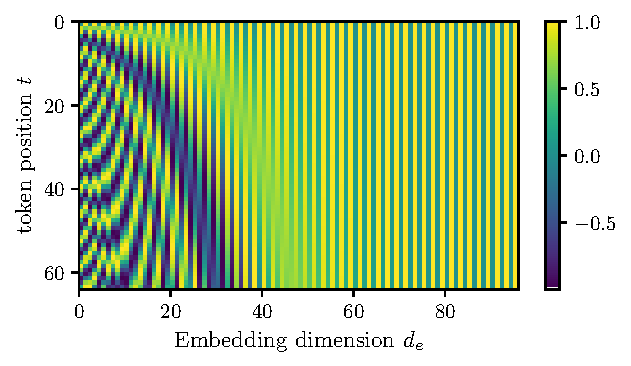
\includegraphics{positional-encoding.pdf}
    \caption[Positional Encoding of Transformer]{Positional encoding. The encoding is added onto the \gls{token} embeddings to infer positional information. The heatmap visualises the uniquely identifying pattern created from sine and cosine signals at increasing frequencies across the embedding dimension.}
    \label{fig:positional-embedding}
\end{figure}

The positional encoding is visualised in \cref{fig:positional-embedding}. One can see the alternating pattern between even and odd columns and the unique pattern for each \gls{token}'s position.

Using trigonometric functions for the positional embedding is favourable, due to being zero-centred and resulting in values in the closed range of $[-1,1]$. These properties are long known to promote convergence of neural networks \autocites[][8-9]{lecunEfficientBackProp2012}[][2]{ioffeBatchNormalizationAccelerating2015}.

The reason for encoding with both the sine and cosine is more subtle, as either one would suffice for absolute embeddings. \textcite[][6]{vaswaniAttentionAllYou2017} hypothesise, that besides learning the \emph{absolute} position i.e., fifth place in sequence, providing both sine and cosine also enables the model to attend to \emph{relative} positions, i.e., two places from a given \gls{token}.

The positional embedding is finally added per element to the token embedding to form a \gls{token}'s initial embedding $\gls{e}$. For the $\gls{t}$-th \gls{token} of a sequence $\mathbf{s}$, the embedding becomes:
\begin{equation}
    \gls{e}=\gls{W-e}\left[:, s[t]\right]+\gls{W-p}\left[:, t\right].
    \label{eq:positional-embedding}
\end{equation}
Intuitionally, adding the positional encoding leads to a rotation of the \gls{token} embedding in the embedding space. As the positional embedding is different for every location within the sequence, otherwise identical \glspl{token}, now have a distinct embedding.

\subsubsection{Attention Mechanism}\label{sec:attention}

Recall from our discussion on token embeddings, that embeddings are not yet context-sensitive. The Transformer relies on an \emph{attention mechanism} to let tokens gather information from other tokens within the sequence and thereby encode the context onto the embeddings.

\textbf{Preliminaries}

Attention can be thought of as a mapping between a query and a set of key-value pairs to an output. In general, the current token is first projected onto a query vector, and all tokens in the context are mapped to key and value vectors. Similar to a soft dictionary lookup, the goal is to retrieve the values from tokens in the context for which the keys are similar to the query and return an aggregate estimate of the values weighted by the similarity of the keys and the query. Naturally, if a token in the context is important for predicting the queried token, indicated by a high similarity, the value of the context token has a large contribution to the output \autocites[][5]{phuongFormalAlgorithmsTransformers2022}[][3]{vaswaniAttentionAllYou2017}.

Attention first appeared in \textcite[][4]{bahdanauNeuralMachineTranslation2016} and was popularised by \textcite[][4]{vaswaniAttentionAllYou2017}. The latter introduced a specific attention mechanism, known as \emph{scaled dot-product attention}, which we introduce in detail.

\textbf{Scaled Dot-Product Attention}

Analogous to before, \emph{scaled dot-product attention} estimates the similarity between queries and keys, as the dot product. The resulting attention scores are divided by some constant and normalised using a softmax function to obtain the attention weights. Multiplication of the attention weights with the values yields the outputs. Scaled dot-product attention is visualised in \cref{fig:transformer-architecture-overview} (left).

For computational efficiency, attention is performed simultaneously over multiple queries. Thus, the author's group queries, keys, and values in matrices. In matrix notation outputs are estimated as:

\begin{equation}
    \begin{aligned}
        \operatorname{Attention}(\mathbf{S},\mathbf{Z}) & = \mathbf{V} \operatorname{softmax}\left(\mathbf{A} / \sqrt{d_{\mathrm{attn}}}\right) \\
        \mathbf{A}                                      & = \mathbf{K}^{\top} \mathbf{Q}
    \end{aligned}
    \label{eq:attention}
\end{equation}
where $\mathbf{S} \in \mathbb{R}^{d_s \times \ell_s}$ and $\mathbf{Z} \in \mathbb{R}^{d_z \times \ell_z}$ are vector representations of the primary input sequence and of the context sequence. Both the primary and the context sequences are identical for the encoder but are different for the decoder. The query, key, and value matrices $\mathbf{Q}=\mathbf{W}_q \mathbf{S} + \mathbf{b}_q\mathbf{1}^{\top}$, $\mathbf{K}=\mathbf{W}_k \mathbf{Z} + \mathbf{b}_k\mathbf{1}^{\top}$, and $\mathbf{V}=\mathbf{W}_v \mathbf{Z} + \mathbf{b}_v\mathbf{1}^{\top}$ are linear projections of the input and context sequences, and $\mathbf{W}_q, \mathbf{W}_k \in \mathbb{R}^{d_{\mathrm{attn}\times d_{s}}}$; $\mathbf{W}_v \in \mathbb{R}^{d_{\mathrm{out}\times d_{z}}}$; $\mathbf{b}_q, \mathbf{b}_k \in \mathbb{R}^{d_{\mathrm{attn}}}$, and $\mathbf{b}_v \in \mathbb{R}^{d_{\mathrm{out}}}$ are learnable parameters. The dimensionality of the attention mechanism, $d_{\mathrm{attn}}$, is typically a fraction of the model dimensionality to accelerate computation. Likewise, the output dimension, $d_{out}$, is another hyperparameter to the models. The attention scores are $\mathbf{A}$, which are scaled by $\sqrt{d_{\mathrm{attn}}}$ to avoid unstable gradients, and the softmax activation normalises all scores. As normalised attention scores have a clear interpretation as the weights of how much a token contributes to the model's output, the attention mechanism provides a window into the model, which we explore in \cref{sec:feature-importance-measure}.

\textbf{Multi-Head Attention}

Rather than relying on a single attention function, \textcite[][4--5]{vaswaniAttentionAllYou2017} introduce multiple \emph{attention heads}, which perform attention in parallel on $H$ \emph{different} linear projections of queries, keys, and values. The \emph{multi-head attention} enables the model to learn richer representations of the input, as attention heads operate independently, they can pick up unique patterns or focus on different positions in the sequence at once. Multi-head attention is visualised in \cref{fig:transformer-architecture-overview} (centre).

Exemplary for machine translation, \textcite[][5795]{voitaAnalyzingMultiHeadSelfAttention2019} show, that heads serve indeed distinct purposes like learning positional or syntactic relations between tokens. It is conceivable, that for tabular data this maps to dependencies between features. In practice, Transformers may not leverage all attention heads and some heads could even be pruned without impacting the performance \autocites[][9]{michelAreSixteenHeads2019}[][5805]{voitaAnalyzingMultiHeadSelfAttention2019}.

Multi-head attention can be computed as:

\begin{equation}
    \begin{aligned}
        \operatorname{MHAttention}(\mathbf{S}, \mathbf{Z}) & = \mathbf{W}_{o}\left[\mathbf{Y}^{1};\mathbf{Y}^{2};\ldots;\mathbf{Y}^{H} \right] + \mathbf{b}_{o}\mathbf{1}^{\top} \\
        \mathbf{Y}^{h}                                     & = \operatorname{Attention}(\mathbf{Q}^h, \mathbf{K}^h, \mathbf{V}^h)
    \end{aligned}
\end{equation}
The query, key, and value matrices  $\mathbf{Q}^{h}=\mathbf{W}^h_q \mathbf{S} + \mathbf{b}^h_q\mathbf{1}^{\top}$, $\mathbf{K}^{h}=\mathbf{W}_k^h \mathbf{Z} + \mathbf{b}_k^h\mathbf{1}^{\top}$, and $\mathbf{V}^{h}=\mathbf{W}_v^h \mathbf{Z} + \mathbf{b}_v^h\mathbf{1}^{\top}$ are obtained from linear projections of the input and context sequences unique per head. Again, $\mathbf{W}^{h}_{q} \in \mathbb{R}^{d_{\mathrm{attn}}\times d_{S}}$; $\mathbf{W}^{h}_{k}, \mathbf{W}^{h}_{v} \in \mathbb{R}^{d_{\mathrm{attn}}\times d_z}$; $\mathbf{b}^h_q, \mathbf{b}^h_k \in \mathbb{R}^{d_{\mathrm{attn}}}$, and $\mathbf{b}^h_v \in \mathbb{R}^{d_{\mathrm{mid}}}$ are used for projection. Typically, the dimensionality of the attention heads, $d_{\mathrm{mid}}$, is reduced to $d_{\mathrm{attn}}/H$ to match the computational cost of single-head attention. The output dimensionality $d_{\mathrm{out}}$ is restored with a final linear projection through the weight matrix $\mathbf{W}_{o} \in \mathbb{R}^{d_{\mathrm{out}}\times Hd_{\mathrm{mid}}}$ and bias $\mathbf{b}_o \in \mathbb{R}^{d_{\mathrm{out}}}$ applied to the concatenated results of the attention heads.

The concatenated and projected output of the attention heads is then passed to the point-wise feed-forward networks, which enables interaction between the head's outputs. We discuss position-wise feed-forward networks in \cref{sec:position-wise-ffn}.

\textbf{Masked Self-Attention and Cross-Attention}

In the \cref{eq:attention}, tokens can attend to any preceding or subsequent token without restrictions. Thus, the full \emph{bidirectional context} is used. This design is optimal for the encoder, where the entire input sequence shall serve as the context.

For the decoder, the self-attention is modified to \emph{masked self-attention} and \emph{cross-attention} mechanism. First, causal masking is required to achieve autoregressive sequence generation in the decoder. The context is \emph{unidirectional}, where a token is only allowed to attend to itself or all previously generated tokens. Second, the decoder uses \emph{cross-attention} to connect between the encoder and decoder. Other than in the self-attention mechanism, where keys, values and queries are generated from the same sequence, keys and values come from the encoder and queries are provided by the decoder. As our focus is on encoder-only architectures, we refer the reader to \textcite[][16--17]{raffelExploringLimitsTransfer2020} for an in-depth treatment of both topics.

\subsubsection{Position-Wise Feed-Forward Networks}\label{sec:position-wise-ffn}

The attention mechanism enables \glspl{token} to attend to other inputs in the immediate context. To retain general information on the task, outside and independent of the immediate context, each Transformer block adds a point-wise \gls{feed-forward-network}, which acts as a persistent memory to the model \autocite[][3]{sukhbaatarAugmentingSelfattentionPersistent2019}.

The network consists of a linear transformation, followed by a non-linear activation function and a second linear layer. For the $l$-th layer, the \gls{MLP} is given by
\begin{equation}
    \mathbf{S} = \mathbf{S}+\mathbf{W}_{\mathrm{mlp} 2}^l \operatorname{ReLU}\left(\mathbf{W}_{\mathrm{mlp} 1}^l \mathbf{S}+\mathbf{b}_{\mathrm{mlp} 1}^l 1^{\top}\right)+\mathbf{b}_{\mathrm{mlp} 2}^l 1^{\top},
\end{equation}
with $\mathbf{W}_{\mathrm{mlp} 1}^l \in \mathbb{R}^{d_{\mathrm{mlp}} \times d_{e}}, \mathbf{b}_{\mathrm{mlp} 1}^l \in \mathbb{R}^{d_{\mathrm{mlp}}}, \mathbf{W}_{\mathrm{mlp} 2}^l \in \mathbb{R}^{d_{e}} \times d_{\mathrm{mlp}}$ and $\mathbf{b}_{\mathrm{mlp} 2}^l \in \mathbb{R}^{d_{e}}$ being learnable parameters identical for all \glspl{embedding} in the layer. The network is applied to each embedding separately and identically.

\textcite[][9]{vaswaniAttentionAllYou2017} set the hidden dimension to be two to eight magnitudes of the embedding dimension. The large capacity strengthens the model's ability to retain information but also contributes significantly to the high computational requirements and memory footprint of Transformers \autocites[][5]{tayEfficientTransformersSurvey2022}[][1]{kitaevReformerEfficientTransformer2020}. Both linear transformations are separated by a \gls{ReLU} \gls{activation-function} \autocite[][318]{glorotDeepSparseRectifier2011} to introduce non-linearities to the network.

Like the attention layer, the position-wise \gls{FFN} is surrounded by residual connections, followed by layer normalisation (cp. \cref{sec:residual-connections-layer-norm}). Both are vital for the training process and convergence of the overall network. Optionally, dropout is added to prevent the model from \gls{overfitting}.

\subsubsection{Residual Connections and Layer Normalisation}\label{sec:residual-connections-layer-norm}

Recall from earlier chapters, that the encoder stacks multiple Transformer blocks, each of which consists of several sub-layers, resulting in a deep network. While depth is inevitable to learn hierarchical representations, the training of such a network is complicated. As neural networks are commonly trained using backpropagation, which relies on the gradient of the error to be propagated through the network starting at the last layer, vanishing or \glspl{exploding-gradient} pose a major difficulty in training deep neural nets \autocite[][1]{heDeepResidualLearning2015}. Without countermeasures, stacking multiple layers in the encoder and decoder of the Transformers impedes the gradient information to flow efficiently through the network and hampers the training behaviour \autocite[][1811]{wangLearningDeepTransformer2019}.

As a remedy, \textcite[][3]{vaswaniAttentionAllYou2017} employ residual connections around each sub-layer, whereby the output of the sub-layer is added element-wisely to its input. Intuitively, the residual connection provides an alternative path for information to flow through the network, since some information can bypass the sub-layer and thereby reach deeper layers within the stack. Vanishing or \glspl{exploding-gradient} are also mitigated, as gradients can bypass the sub-layer, eventually contributing towards an easier optimisation \autocite[][3591]{liuRethinkingSkipConnection2020}. Residual connections moreover help to preserve the positional embeddings (cp. \cref{sec:positional-encoding}), as the layer's inputs are maintained in the identity mapping. Another technique to improve the training behaviour is layer normalisation.

\textcite[][3]{vaswaniAttentionAllYou2017} extensively draw on layer normalisation \autocite[][4]{baLayerNormalization2016} after the multi-head attention and feed-forward sub-layers. It is used for normalising the activations of the sub-layer and to stabilise and accelerate the training of the network \autocite[][2]{baLayerNormalization2016}. The normalisation statistics are calculated separately for every instance, which guarantees scalability across different batch sizes.

Until now it remains unclear, how the layer normalisation intertwines with the sub-layers and the residual connections. Transformers are distinguished by the order in which layer normalisation is added into the pre-norm and post-norm Transformer. Post-norm Transformers add layer normalisation to the sub-layer \emph{after} adding the input from the residual connections. The arrangement is depicted in \cref{fig:transformer-architecture-overview}. In contrast for pre-norm Transformers, the normalisation is applied \emph{before} the self-attention and feed-forward sub-layers and inside the residual connections. Pre-norm requires one additional normalisation layer to pass only well-conditioned outputs from the Transformer block to the successive layers \autocite[][5]{xiongLayerNormalizationTransformer2020}.

\textcite[][3]{vaswaniAttentionAllYou2017} employ post-layer normalisation, but recent research has shown a shift towards pre-norm setups \autocite[][4]{narangTransformerModificationsTransfer2021}. Parts of the widespread adaption lie in faster training and omitting of the need for costly learning rate warm-up stages, whereby the learning rate is initially decreased to keep the gradients balanced \autocites[][2]{xiongLayerNormalizationTransformer2020}[][8]{liuUnderstandingDifficultyTraining2020}. In addition, post-norm Transformers have been found brittle to train and prone to convergence failures with its root cause in vanishing gradients, \glspl{exploding-gradient}, and an overall higher dependency on the residual stream \autocites[][8]{liuUnderstandingDifficultyTraining2020}[][1812]{wangLearningDeepTransformer2019}. Pre-norm Transformers, although they may sacrifice some performance, introduce a certain robustness to the training process. We come back to this property in our discussion on the FT-Transformer.

\subsubsection{FT-Transformer}\label{sec:fttransformer}

\todo{try to introduce BERT here somewhere.}

Many of the previous concepts can be adapted to the tabular domain with minor architectural changes. \textcite[][5]{gorishniyRevisitingDeepLearning2021} propose with FT-Transformer an adaption, that pairs an embedding unit for both numerical and categorical inputs, dubbed the feature tokenizer, with a Transformer. The complete architecture is depicted in \cref{fig:fttransformer}. Notably, the Transformer units use a pre-norm setup for easier optimisation, whereby the very first normalisation layer in the encoder is removed due to a propitious performance \textcite[][17]{gorishniyRevisitingDeepLearning2021}. The upstream feature tokenizer transforms every feature in $\mathbf{x}$ to their embeddings. The embeddings are given by \cref{eq:numerical-embeddings,eq:categorical-embeddings}.

\begin{figure}[ht]
    \centering
    {\renewcommand\normalsize{\scriptsize}
        \normalsize
        \input{./Graphs/fttransformer.pdf_tex}}
    \caption[Overview Over the FT-Transformer Architecture]{Overview Over the Architecture of FT-Transformer. The FT-Transformer uses a pre-norm arrangement and operates on numerical and categorical embeddings. Own work inspired by \textcite[][4--5]{gorishniyRevisitingDeepLearning2021}.}
    \label{fig:fttransformer}
\end{figure}

Recall from our discussion on self-attention (cp. \cref{sec:attention}), that each \gls{token} encodes the \glspl{token} within the sequence. Based on this notion, \textcite[][4174]{devlinBERTPretrainingDeep2019} prepend a specialised $\mathtt{[CLS]}$ \gls{token} to the sequence, which stores the sequence's aggregate representation. Like any other \gls{token}, the $\mathtt{[CLS]}$ \gls{token} is embedded first and contextualised in the encoder. Its final hidden state is then used for classification.

\textcite[][4]{gorishniyRevisitingDeepLearning2021} adapt the idea of a $\mathtt{[CLS]}$ \gls{token} for tabular representation models. Similar to the embeddings of categorical or numerical features, the embedding of the $[\mathtt{CLS}]$ \gls{token} $\gls{e}_\mathtt{[CLS]} \in \mathbb{R}^{d_{e}}$ is prepended to the column embeddings with $\mathbf{S} = \left[\gls{e}_\mathtt{[CLS]}, \gls{e}_1, \ldots \gls{e}_{M}\right]$, where $\mathbf{S} \in \mathbb{R}^{d_{e} \times M +1}$. Like before, $\mathbf{S}$ is passed through a stack of Transformer layers. The updated representation of the $\mathtt{[CLS]}$ \gls{token} is used exclusively for prediction:
\begin{equation}
    P=\operatorname{Linear}\left(\operatorname{ReLU}\left(\operatorname{LayerNorm}\left(\mathbf{S}\left[:,0\right]\right)\right)\right).
    \label{eq:bert-ft}
\end{equation}
\todo{Add softmax, think about ReLU, change linear layer to Weight matrix?}

\textcite[][8]{gorishniyRevisitingDeepLearning2021} achieve state-of-the-art performance through numerical and categorical embeddings. Embedding both categorical and numerical inputs enables the Transformer to attend to all other features, but at considerable computational cost, that may only be justified by higher classification accuracies.

Next, all models are extended for learning on partially-labelled data.